\section{End-to-end framework}
%%%%%%%%%%%%%%%%%%%%%%%%%%%%%%%%%%%%%%%%
\begin{figure*}[htp!]
\centering
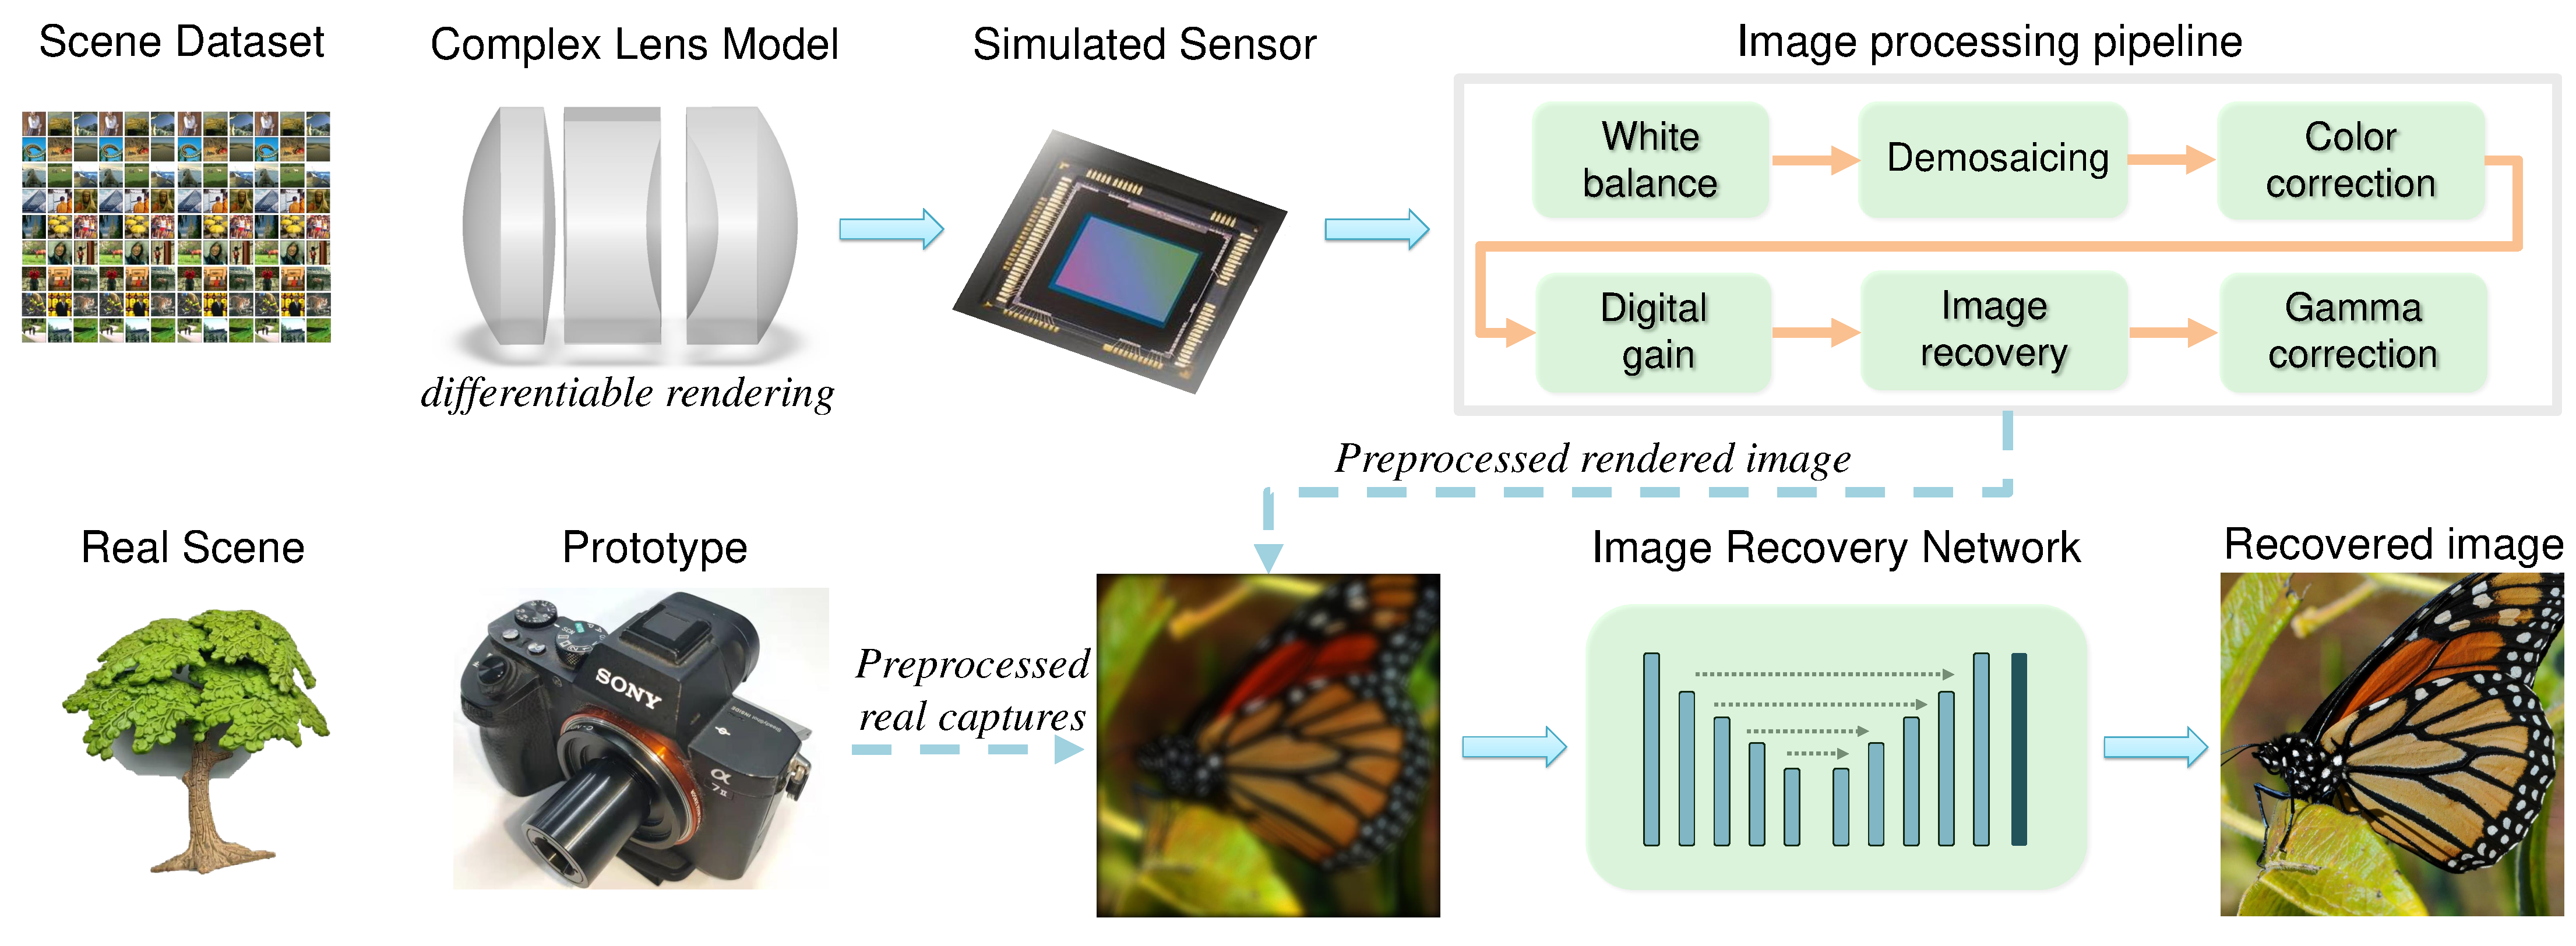
\includegraphics[width=2.1\columnwidth]{figures/E2ELearning.pdf}
    \vspace{-18pt}
\caption{Framework for joint learning of differentiable complex lens model and reconstruction. We set the 
 In each forward pass, the synthetic PSF is convolved with a batch of images, and Poisson noise is added to account for sensor's counting noise after the interval sampling process.
After obtaining the optimized PSF, we apply a Gerchberg-Saxton-based phase retrieval algorithm to derive the phase mask. The reconstruction network is composed of three main parts: initial feature extraction, back projection stages, and reconstruction step. The back-projection stage (right bottom), alternating between reconstruction of $H^t$ and $L^t$, consists of $T$ up projection stages and $T-1$ down projection stages. Each unit is connected with the outputs of all previous units.}
\label{fig:framework}
   \vspace{-5pt}
\end{figure*}

We aim to realize super-resolution imaging over a SPAD sensor that
suffers from both low resolution and low fill-factor.  These two
problems will result in significant spatial aliasing and the
associated reconstruction artifacts~\cite{Parker:2017:DSP:3152597}.
To address this issue, we introduce an optical low-pass filter (OLPF)
into the optical system of the camera. The OLPF acts as an
, that is specially designed to suppress
aliasing while preserving as much information as possible for
super-resolution image reconstruction.

After training, we extract the optimal PSF from the weights of
$conv(11,1)$ and then apply a Gerchberg-Saxton (GS)-based phase
retrieval algorithm to derive the phase mask (see left-bottom of
Figure~\ref{fig:framework}), which acts as an optical coder installed
at the front focal plane of a regular lens to generate the optimal PSF
for later implementations. In order to account for differences between
the design and the fabrication of the phase mask, the real-world PSF
of the mask can be calibrated, and the reconstruction network can be
fine-tuned through re-training.

In the following, we first detail the image formation model,
incorporating the anti-aliasing filter applied to the sampling model
of SPAD array and the phase mask optimization to generate the learned
PSF combined with a regular imaging lens. Next, we present the deep neural
network reconstruction and the time profile sharpening strategy.


\subsection{Image Formation}
%%-----------------------------------------------------------

\subsubsection{Anti-aliasing filtering and image sampling}
\label{sec:SamplingModel}
As mentioned, the fill factor of most current SPAD imaging sensors is
very low, that is, the light sensitive area of the pixel is much
smaller than the total area occupied by the pixel structure.  For
example, the SPAD array used in our experiments (MPD-SPC3) has a pixel
pitch of 150~$\mu$m horizontally and vertically, however the active
area is only 30~$\mu$m in each dimension. The physical low pixel count
and small fill-factor severely degrade the image quality, creating the
desire for super-resolved image reconstruction. To avoid aliasing, the
image signal should be pre-filtered with a low pass filter of the
appropriate cut-off frequency, followed by a down-sampling
process~\cite{Parker:2017:DSP:3152597}. Again, the goal is to
trade-off sharpness and aliasing, so as to find a good compromise that
preserves most details of interest.

Due to the low resolution of the sensor array, we can
 reasonably neglect off-axis aberrations like coma.
Image formation becomes a shift-invariant convolution of a latent
image with a kernel. To this end, we jointly learn the optimal
anti-aliasing filter (e.g. the convolved kernel) and the
reconstruction network to eventually preserve the finest details of
natural images so as to realize a super-resolution enhancement.  The
quantitative evaluation of applying this desired OLPF is detailed in
Section~\ref{sec:simulation}.

At the position $(x,y)$ on the sensor, the detected signal $I_s(x,y)$
is expressed as:
\begin{equation}\label{eq:imagingModel}
I_s(x,y)=\mathcal{P}  ( \mathcal{S}  ( \bm{p}_{\lambda}*\bm{I} ) ),
\end{equation}
where $\mathcal{S}$ is a 2D sampling operator corresponding to the
physical structure of SPAD sensor, $\bm{I}$ is the latent image formed
on the sensor, $\bm{p}_{\lambda}$ is the kernel (or PSF) realized by
the optical system, and $\mathcal{P}$ represents a generator of the
Poisson noise, which is the appropriate noise model for low light
scenarios that are typical for SPAD imaging.


\subsubsection{Learning optimal PSF using end-to-end design}
To obtain the optimal PSF $\bm{p}_{\lambda \text{opt}}$ using our
end-to-end framework, we model our PSF as well as the low-resolution
sampling process of the SPAD array as a convolutional layer
$conv(11,1)$.
%\todo{the footnote should go here, or be included in the main text.}
In each forward pass, the synthetic PSF (convolutional layer)
is convolved with a batch of images, and Poisson noise is added to
account for photon shot noise after the interval sampling
process. In other words, we represent both the PSF and the sampling
process as layers in our neural network during training, and then
physically realize the learned result as a custom DOE  for our SPAD
camera (see Section~\ref{sec:maskgen}).

To determine the size of the kernel,
we take a large kernel  $21\times 21$ at the beginning and then we found 
only an $11\times11$ region of the filter had non-zero values. Therefore, 
we take $11\times11$ as the kernel size of the PSF whose physical dimension
is $412.5\times412.5 \mu m^2$.

\subsection{Image Reconstruction}
\label{sec:Reconstruction}

Image reconstruction is the final stage for applications like regular
intensity imaging or high speed imaging, and the second last stage for
applications like depth and transient imaging.  For our camera the
reconstruction is formulated as an optimization problem of a data
fitting term with an additional regularization term:
\begin{equation}\label{eq:costfunction}
\min_{\bm{I}} \frac{1}{2}\| \mathcal{S}(   \bm{p}_{\lambda \text{opt}}*\bm{I}) - \bm{I}_s \|_2^2+ 
\beta\| \Phi(\bm{I}) \|_1,
\end{equation}
where $ \Phi(\cdot)$ denotes the transform coefficients of $\bm{I}$
with respect to some transform $\Phi$ that can be either linear or
optimized non-linear. Sparsity in the transform space
$\Phi(\bm{I})$ is encouraged by the $\ell_1$ norm with $\beta$ being a
regularization parameter.

Usually, natural images are non-stationary in classic domains like
DCT, gradients, and wavelets, which may result in an ill-posed problem
under such an imaging model. Although an optimized PSF model can
preserve a large amount of spatial information, conventional
optimization-based methods fail to faithfully reconstruct good quality
results when the sampling ratio is very low (e.g. in our case with a
sampling ratio only 3.14$\%$). To this end, a trainable architecture
for super-resolution with powerful learning ability for features meets
our strict requirements as our learned PSF itself encodes features. We
choose the state-of-the-art method--- dense deep back-projection
networks (D-DBPN)~\cite{haris2018deep} as our reconstruction network,
as shown in Figure~\ref{fig:framework}. The D-DBPN framework
introduces an iterative error correcting feedback mechanism to
characterize the features in previous layers. More importantly, it
addresses the mutual dependency by taking the back-projection from HR
domain to LR domain.

\subsubsection{Framework architecture}
As shown in Figure~\ref{fig:framework}, the end-to-end framework 
to obtain the optimal filter and reconstruction network can
be divided into four parts: 

\paragraph{a. Imaging model.} As we have already discussed in Sec.~\ref{sec:SamplingModel},
we take the physical imaging model as the first part of our end-to-end
framework. The joint framework is used to learn the optimal
anti-aliasing filter.  After fabricating the filter we then refine the
learning process of the reconstruction network with additional
training to account for fabrication errors. For more details, please
refer to Section~\ref{sec:Prototype}.

\paragraph{b. Initial feature extraction.}
The initial feature maps $L^0$ are constructed using a $conv(3, n_0)$
layer to extract features and a $conv(1, n_R)$ layer to pool the
features and reduce the dimension from $n_0$ to $n_R$. In the
experiments, $n_0$ is set as 256 and $n_R$, which is the number of
filters used in each projection unit, is set as 64.

\paragraph{c. Back-projection.}
As illustrated in Figure~\ref{fig:framework}, at $t^{th}$ stage
($T=7$ stages in total), the LR feature maps
$[L^1,L^2,\cdots,L^{t-1}]$ and HR feature maps $[H^1,H^2,\cdots,H^t]$
are concatenated to be used as input for up- and down-projection units
respectively. In each projection unit, we use a $conv(1, n_R)$ to
merge all previous outputs from each unit after the shown
concatenation process.

The up-projection is defined as follows:
\begin{equation}
\label{eq:up-projection}
\begin{alignedat}{2}  &\text{scale up}  \ \ \ \  && H_0^t = conv^T(f_p, n_R)[L^{t-1}]\\
 &\text{scale down}   \ \ \ \ \ &&  L_0^t = conv(f_p, n_R)[H_0^{t}] \\
 &\text{residual: } && e^l_t = L_0^t - L^{t-1}\\
 &\text{scale residual up:\,} && H_1^t = conv^T(f_p, n_R)[e_t^l] \\
 &\text{output feature map:\,} && H^t = H^t_0 + H^t_1
\end{alignedat}
\end{equation}

The down-projection is defined as follows:
\begin{equation}
\label{eq:down-projection}
\begin{alignedat}{2}  &\text{scale down}  \ \ \ \  && L_0^t = conv(f_p, n_R)[H^{t}]\\
 &\text{scale up}   \ \ \ \ \ && H_0^t = conv^T(f_p, n_R)[L_0^{t}] \\
 &\text{residual: } && e^h_t = H_0^t - H^{t}\\
 &\text{scale residual down:\,} && L_1^t = conv(f_p, n_R)[e_H^l] \\
 &\text{output feature map:\,} && L^t = L^t_0 + L^t_1
\end{alignedat}
\end{equation}

\paragraph{d. Reconstruction.}
Finally, we take the concatenated HR feature maps
$[H^1,H^2,\cdots,H^t]$ as input and use a $conv(3, 1)$ layer to
reconstruct the target HR image.
 
 \subsubsection{Training details}
 To train the network, we use the mean square error (MSE) loss
 function.  In the stated framework, we use an 8$\times$8
 convolutional layer with a stride of four and a padding of two. All
 convolutional and transposed convolutional layers are followed by a
 parametric rectified linear unit. We trained our network using the
 high resolution images from the DIV2K dataset, using a batch size of
 64. For convenience, the LR image resolution was 32$\times$32 (half
 the size of our SPAD array), and the HR image size was
 128$\times$128.  We take a convolution layer $conv(11,1)$ as our PSF
 following the sampling model of the SPAD sensor to simulate the LR
 images from HR images.  We use ADAM as the optimizer with momentum
 set to 0.9 and weight decay set to $10^{-4}$.  The learning rate is
 initialized to $10^{-4}$ for all layers and decayed by a factor of 10
 for every half of total epochs. All experiments were conducted using
 Pytorch on a single NVIDIA TITAN Xp GPU. For learning the optimal
 PSF, we trained the whole framework with 50 epochs taking around 40
 hours. After calibrating the PSF generated by the fabricated phase
 mask, we take the weights of the network trained above as
 initialization and continue to train the reconstruction network with
 11 epochs taking around 8 hours.



\subsection{Phase Mask Generation}
\label{sec:maskgen}
After obtaining the optimal PSF with our framework, we establish
the relationship between the PSF and the phase mask. We first
analyze the propagation of light from the phase mask to the image
plane,  and then present the details of phase mask design. 

\subsubsection{Optical model}
As shown in Figure~\ref{fig:PSFMODEL}, the mask is placed at
the front focal plane of the lens, and acts as the pupil of whole
system.
For modeling the light propagation, we apply scalar diffraction
theory~\cite{goodman2005introduction} to approximate the paraxial
incident wave.  The phase of a complex-valued incident wave is delayed
by a phase profile $\phi(x',y')$ proportionally to the height map of a
diffractive optical element $h(x',y')$:
\begin{equation}\label{eq:phase_height}
\phi(x',y') = \Delta n \frac{2\pi}{\lambda} h(x',y'),
\end{equation}
where $\lambda$ is the wavelength, $(x', y')$ is the location on the
phase mask plane , and $\Delta n = n-n_0$ represents the refractive
index difference between air ($n_0$) and the substrate material
($n$). Placed at the front focal plane of a lens together with our
customized limited stop, the phase mask acts as the complex pupil
function.

The incident wave field $U_{\lambda}(x',y',z=0_-) = A(x',
y')\phi_d(x',y')$ is modulated by the phase mask, shown as:
\begin{equation}\label{eq:incident_wave}
U_{\lambda}(x', y', z = 0_+) = U_{\lambda}(x',y',z=0_-) \cdot e^{\mathbf{i}\phi(x', y')},
\end{equation} 
where we use the notation $z=0_-$ and $z=0_+$ to denote positions just
before and just after the mask, respectively.


Using the Fresnel approximation, the light propagates through a lens
with a focal length $f$ to the image plane is then formulated as:
\begin{equation}
\label{eq:diffractionZ}
\begin{alignedat}{1}U_{\lambda}(x,y)= & \frac{e^{\mathbf{i}kf} } {\mathbf{i}\lambda f } \int\int_{\sum}
U_{\lambda}(x', y', z=f) e^{ -\frac{\mathbf{i}k}{2f} (x'^{2}+y'^{2}) }\\
 & e^ { \frac{\mathbf{i}k}{2f} \left[(x-x')^{2}+(y-y')^{2}\right] } dx'dy' \\
 &=  \int\int_{\sum} \phi(x', y') e^{ -i2\pi \frac{x'x+y'y'}{\lambda f} }dx'dy',
\end{alignedat}
\end{equation}
where $k=2\pi/\lambda$ is the wave number, $(x, y)$ is the location
on the image plane, and $e^{ -\frac{\mathbf{i}k}{2f} (x'^{2}+y'^{2}) }$ represents the optical transfer function of the lens. Note that Equation (\ref{eq:diffractionZ}) represents
essentially a Fourier transform (FT).


For an imaging system, the diffractive PSF on the image plane is
eventually obtained as:
\begin{equation}\label{eq:phase2PSF}
p_{\lambda}(x,y) \propto \| (\mathcal{F}\{\phi(x',y') \} \|^2.
\end{equation}
\subsubsection{Phase retrieval}
After deriving the relationship between PSF and the phase mask, we can
design a physical height profile $h(x', y')$ on a substrate of
refractive index $n$ to implement an image-plane PSF
$\bm{p}_{\lambda}$ using the Gerchberg-Saxton (GS)~\cite{GS1972} phase
retrieval algorithm based on Equation~(\ref{eq:phase_height}).

The core of the phase retrieval is shown on the bottom left of
Figure~\ref{fig:framework}. In the beginning, a random phase
distribution serves as the initial estimate subject to the amplitude
of the PSF.  Then, using the initial phase and the amplitude
constraint (between 0 and 1) of learned PSF, we apply an inverse
Fourier transform on this synthesized complex field function.  The
resulting phase part of the discrete complex field is preserved while
the amplitude part is discarded. In the next round, this preserved
phase is plugged into the forward propagation procedure of applying a
Fourier transform to update the amplitude estimate of the complex
field on the image plane.  Eventually, the process is repeated with a
finite number times to converge to an optimal phase profile. For more
details, please refer to the work by Morgan et
al.~\shortcite{morgan2004development}. Since we optimize the
  phase plate for only one wavelength (that of our picosecond laser),
  we are guaranteed to obtain a phase plate that can generate the
  optimal PSF we desire. As shown in Figure~\ref{fig:GS}, the
  correlation coefficient between the PSF generated by phase plate and
  the learned PSF is 0.9996, and the RMSE between them is 0.0061. This
  all means the optimal PSF is accurately realized by the phase mask.
 


\subsubsection{Phase mask tiling}
\label{sec:phaskMaskDesign}
As shown in Figure~\ref{fig:calibratedPSF}, a subpixel on the learned
PSF has a size of $l_{p}$ = 37.5~$\mu$m. Accordingly, the size of
phase profile obtained using Equation~\ref{eq:diffractionZ} is $l_{u}
= \lambda f / l_{p} = 0.8733$~mm, which would make for a very small,
square aperture. To design optical systems with larger apertures, one
could over-parameterize the design space to optimize the phase profile
over a defined larger aperture. This would require a re-design of the
pattern for each aperture size, and rule out the use of the aperture
stop diaphragm in the main camera lens.

 

A simple alternative that overcomes these issues, is to side-by-side
replicate the small optimized phase pattern described above in order
to tile the aperture. In our prototype, we tile a square area of edge
length $L=14$~mm, which defines a maximum aperture that can be further
stopped down using the lens diaphragm.  The tiling has the effect of
creating a discrete dot pattern instead of a continuous PSF in the
image plane. At a size of $l_{p} l_{u}/L=$ 2.34~$\mu$m, the individual
dots are significantly smaller than a sub-pixel and their
center-to-center spacing is exactly the sub-pixel pitch, which also
matches the edge length of the light sensitive area of a SPAD
pixel. Therefore, as the SPAD sensor integrates spatially over the
light sensitive area, it integrates over exactly one of the dots in
the dot pattern, which is equivalent to implementing the continuous
version of the PSF designed above.

As an added benefit, the dot pattern simplifies the alignment process
in the assembly of the optical system. As illustrated in
Figure~\ref{fig:calibratedPSF},(d1)-(d3), slight defocus does not
spread the energy out of the subpixel block. If we were to instead
employ a large, non-repeating mask, a slight slight defocus would
spread energy to neighboring subpixels, equivalent to an additional
low-pass filter, as illustrated in
Figure~\ref{fig:calibratedPSF},(d4)-(d5).

\subsection{Temporal Sharpening for Depth and Transient Imaging}
To extract temporal information from our reconstructed images, we
use a recent reported temporal PSF model~\cite{sun2018depth} for SPAD
sensors to sharpen our reconstructed 3D data.  For depth and transient
imaging, our SPAD sensor works in time-correlated single photon
counting (TCSPC) mode.

This model is useful for precise temporal localization of
  Gaussian laser pulses from an observed time profile at each pixel
  $\bm{I_i}$, using a model of the temporal response of the SPAD
  pixel, $\bm{\Pi}(t)$. The gate signal $\bm{\Pi}(t)$ is not a simple
  rectangular pulse, but is distorted according to a
  resistor-capacitor (RC) circuit response (also compare
  Figure~\ref{fig:fitting} bottom left). We band limit this RC model
  with a small Gaussian filter ($\sigma_f=$~100~ps in the
  experiments), see Figure~\ref{fig:fitting} bottom center.  

 The observed time profile at each pixel $\bm{I_i}$ is then
  modeled as a convolution of this gate model $\bm{\Pi}(t)$ with the
  Gaussian laser pulse
  $\bm{G}(t;A,\mu)=A\bm{e}^{-\frac{(t-\mu)^2}{2\sigma^2}}$, where the
  parameters $A$ and $\mu$ of the Gaussian are initially unknown. They
can be determined by solving the following minimization problem for
each pixel:

\begin{equation}
  \label{eqn:psfmodel}
  \min_{A,\mu} \|\mathbf{G}(t;A,\mu)\ast \bm{\Pi}(t) - \bm{I_i} \|_2^2,
\end{equation}
 where $\ast$ denotes the convolution. Please refer to the
  original paper of Sun et al.~\shortcite{sun2018depth} for technical
  details. Instead of using a Gaussian model for the laser pulse, we
  note that it would be straightforward to substitute other models
  such as an exponentially modified Gaussian~\cite{heide2014imaging}
  to estimate parameters for inter-reflection, subsurface scattering,
  or fluorescent lifetime imaging (FLIM).
 
 

% --- DO NOT DELETE ---
% Local Variables:
% mode: latex
% mode: flyspell
% mode: TeX-PDF
% End:

